\documentclass{beamer}
\usepackage{ngerman}
% \usepackage{beamerthemelgdv}
\usepackage{lgdv/beamerthemetest}
\usepackage[utf8]{inputenc}
\usepackage{subfigure}
\usepackage{listings}



\title{GraPRA}
\subtitle{Wintersemester 2014}
\author{Team 6\\Oliver Brehm, Judith Hemp, Daniel Schröder}
\date{30.01.2015}

\newcommand{\TODO}[1]{{\large\bf Todo: #1}}

\subject{GraPra}	% goes to pdf meta
\keywords{Computer Graphics, Slides created with LaTeX}	% dito

\begin{document}

\frame{\titlepage}

% \usebackgroundtemplate{}
\newcommand{\slide}[2]{\frame{\frametitle{#1} #2}}
\newcommand{\topic}[1]{\frame{\begin{center}\huge\rm\textbf{#1}\end{center}}}

\slide{Pacman VS Bomberman Wars}{
        \begin{center}
        
\includegraphics[width=.5\paperwidth]{nochicks}%awesome gameplay pic
        \end{center}
}

\slide{Pacman VS Bomberman Wars}{
        \begin{itemize}
        \item Inspired by previous Grapra assignments
        \item Simple strategy game
        \item Multiplayer network game (no AI)
        \end{itemize}
}

\slide{Tenchnical overview}{
        \begin{itemize}
        \item Client-Server architecture
        \item Terrain rendering using a heightmap with tessilation
        \item Tilebased world map on the logic side
        \item Pathfinding using a star
        \vskip1cm
        \end{itemize}
}

\slide{Building types: Construction sites}{
        \begin{center}
        
\includegraphics[width=.5\paperwidth]{nochicks}%Constr site pic
        \end{center}
        \begin{itemize}
        \item Construction sites belong to no player
        \item Send 10 units to create a building
        \end{itemize}
}

\slide{Building types: Settlements}{
        \begin{columns}
                \column{.4\paperwidth}
                        \centering
                        
\includegraphics[width=.3\paperwidth]{nochicks} % Settlement 1 pic%
                \column{.4\paperwidth}
                        \centering
                        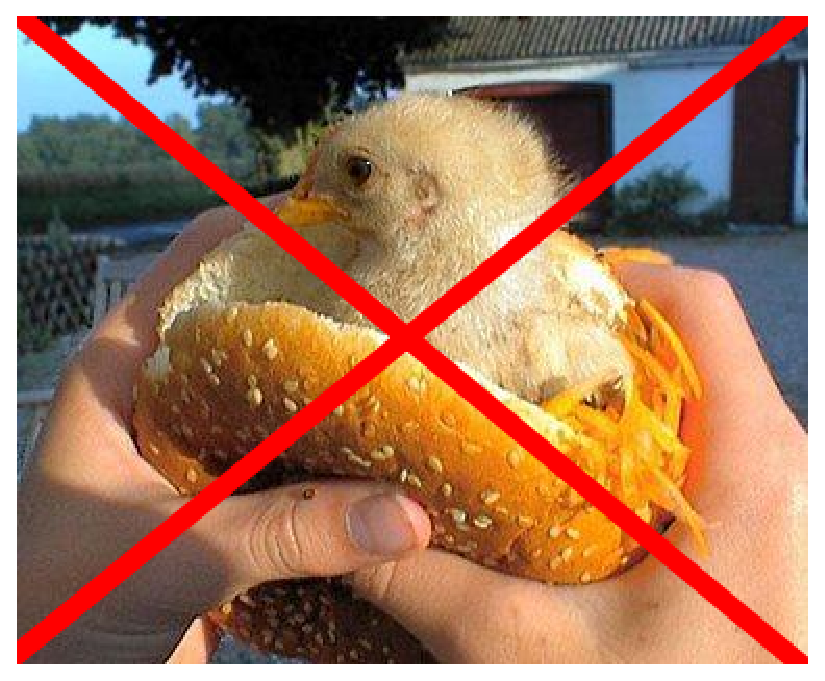
\includegraphics[width=.3\paperwidth]{noviolence} %Settlement 2 pic%
        \end{columns}
        \begin{itemize}
        \item Different levels of player settlements
        \item Higher level settlements produce more units
        \end{itemize}
}

\slide{Building types: Turrets}{
        \begin{columns}
                \column{.4\paperwidth}
                        \centering
                        
\includegraphics[width=.3\paperwidth]{nochicks} %Turret 1 pic%
                \column{.4\paperwidth}
                        \centering
                        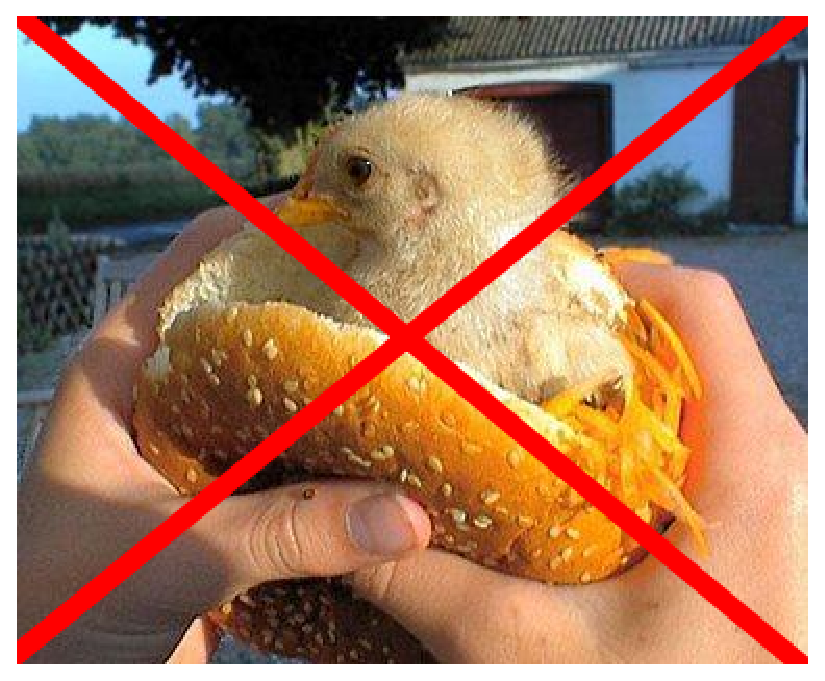
\includegraphics[width=.3\paperwidth]{noviolence} %
        \end{columns}
        \begin{itemize}
        \item Different levels of turrets
        \item Turrets produce no units but are harder to attack
        \end{itemize}
}

\slide{GUI overlay for upgrading}{
        \begin{center}
        
\includegraphics[width=.5\paperwidth]{nochicks}%gui overlay pic
        \end{center}
}

\slide{Sending troups}{
        \begin{columns}
                \column{.4\paperwidth}
                        \centering
                        
\includegraphics[width=.3\paperwidth]{nochicks}%Selection pic%
                \column{.4\paperwidth}
                        \centering
                        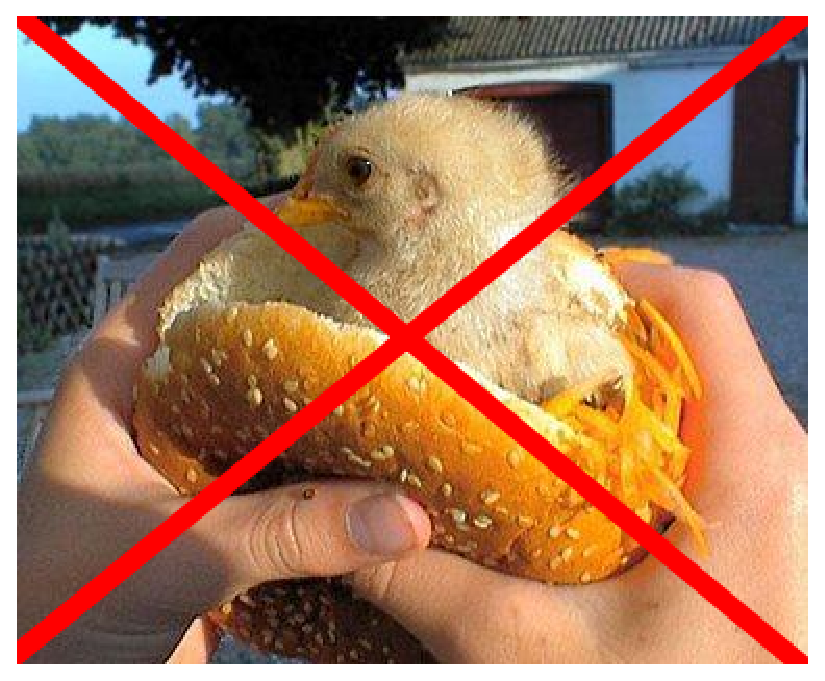
\includegraphics[width=.3\paperwidth]{noviolence}%amount slider pic%

        \end{columns}
        \begin{itemize}
        \item First select your own building
        \item Select destination building and amount of units to send
        \end{itemize}
}

\slide{Incoming troups}{
        \begin{columns}
                \column{.4\paperwidth}
                        \centering
                        
\includegraphics[width=.3\paperwidth]{nochicks} % moving troups pic%
                \column{.4\paperwidth}
                        \centering
                        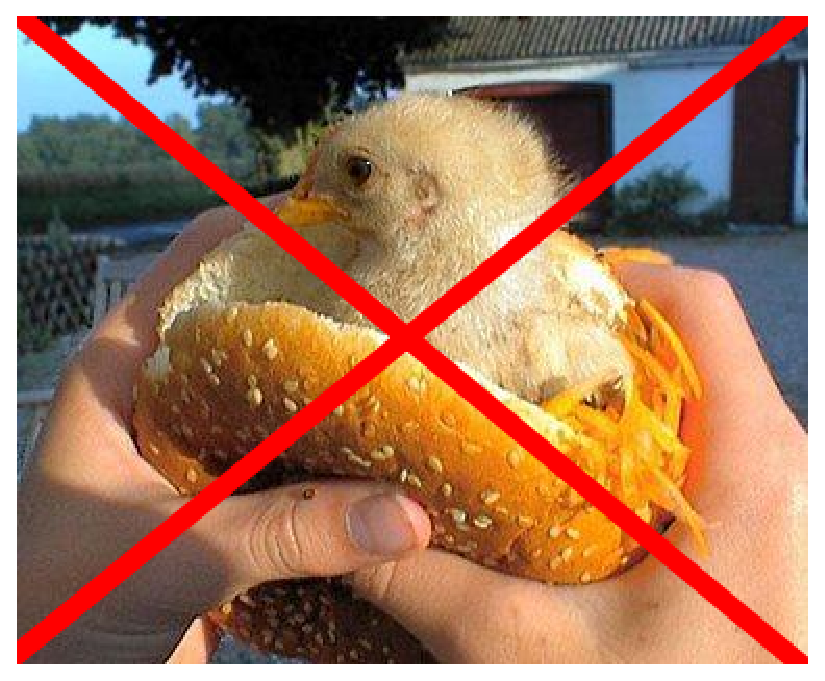
\includegraphics[width=.3\paperwidth]{noviolence} % incoming troups pic%
        \end{columns}
        \begin{itemize}
        \item Units move in small groups
        \item If you send enough units, the enemy building will be yours
        \end{itemize}
}

\slide{Video}{
        \begin{center}
        % \Huge\bf\tt blub
        Pacman and Bomberman in action
        \end{center}
}

\slide{\ }{
	\begin{center}
        Thanks for listening and have fun playing!
	\end{center}
}

\end{document}

